%=========================================================
% Exceptions 
%=========================================================
\section{Exceptions}

Privileged mode of mmRISC-1 is only Machine-Mode (M-Mode). Exceptions are divided into two categories; one is synchronous exceptions which are invoked by instructions, and the other is asynchronous exceptions which are invoked by interrupt inputs.\\
Whenever an exception occurs, hardware will automatically save and restore important registers. The following steps are completed by hardware before jumping to the vector which corresponds to each exception.

\begin{enumerate}
    \item Save PC to MEPC.
    \item Save Privilege level to MSTATUS. (Fixed to 2 due to only M-Mode is supported.)
    \item Save MSTATUS.mie to MSTATUS.mpie.
    \item Disable interrupts by setting MSTATUS.mie = 0.
    \item MTVAL is set to specific data corresponding to each exception.
    \item MCAUSE is set to cause information corresponding to each exception.
    \item Set PC to corresponding exception’s Vector Address associated to MTVEC (Direct Mode or Vectored Mode).
\end{enumerate}

At this point, software receives its responsibility to handle proper exception process. After the process is finished, the MRET instruction should be executed. The MRET executes following steps.

\begin{enumerate}
    \item Restore MSTATUS.mpp to privilege level. (Fixed to 2 due to only M-Mode is supported.)
    \item Restore MSTATUS.mpie to MSTATUS.mie.
    \item Restore MEPC to PC.
\end{enumerate}

Supported exceptions and corresponding MCAUSE, Vector Address and MTVAL are summarized in Table \ref{tb:EXCEPTION_LIST}. If an instruction invokes multiple synchronous exceptions simultaneously, one of those is selected by priorities shown in Table \ref{tb:EXCEPTION_PRIORITY}.

\begin{table}[H]
    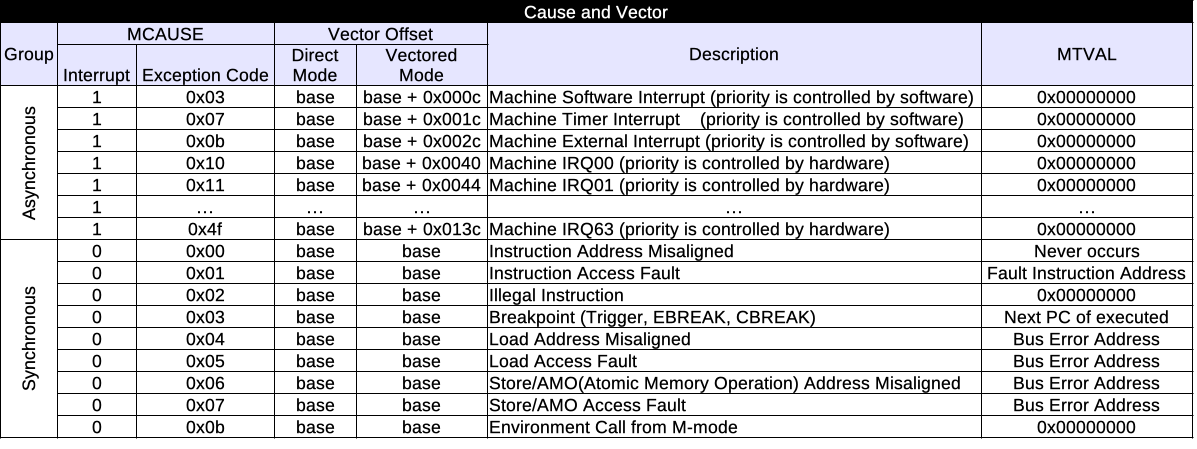
\includegraphics[width=1.00\columnwidth]{./Table/Exception_List.png}
    \caption{Exceptions}
    \label{tb:EXCEPTION_LIST}
\end{table}

\begin{table}[H]
    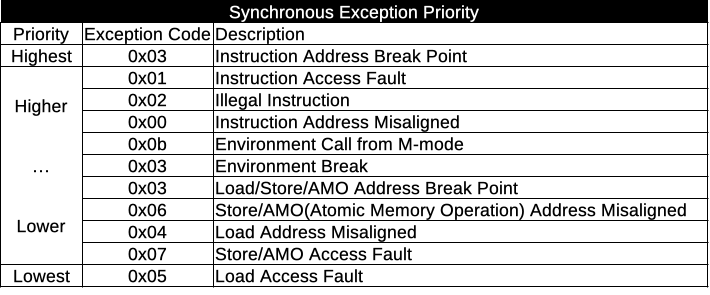
\includegraphics[width=1.00\columnwidth]{./Table/Exception_Priority.png}
    \caption{Priority of Synchronous Exception}
    \label{tb:EXCEPTION_PRIORITY}
\end{table}





